\documentclass[12pt]{article}

% Setting up the page
\usepackage[margin=20mm,includefoot,footskip=10mm]{geometry}
\usepackage{setspace}
    \onehalfspacing%

% Bibliography, referencing
\usepackage[numbers]{natbib}
    \bibliographystyle{abbrvurl}
\usepackage{hyperref}

% Mathematics, symbols
\usepackage{amsmath}
    \DeclareMathOperator*{\argmin}{arg\,min}
\usepackage{pgf, interval}
    \intervalconfig{soft open fences}

% Images, tables
\usepackage{graphicx}
    \graphicspath{{img/}}
\usepackage{booktabs}
    \renewcommand{\arraystretch}{1.3}
\usepackage{caption}
\usepackage{subcaption}

% Mathematics
\usepackage{amssymb}

% Custom lengths
\newlength{\imgwidth}
\setlength{\imgwidth}{.9\textwidth}
\newlength{\tabwidth}
\setlength{\tabwidth}{.9\textwidth}

\title{%
    Understanding COPD patients in the hospital system via administrative data
}
\author{Henry Wilde, Vincent Knight, Jonathan Gillard}
\date{}


\begin{document}
\maketitle%

\begin{abstract}
    This work presents an analysis of how patients with chronic obstructive
    pulmonary disorder (COPD) interact with the hospital system in South Wales.
\end{abstract}

\section{Introduction}\label{sec:intro}

Population health research is becoming increasingly based on data-driven methods
(as opposed to those designed solely by clinical experts) for patient-centred
care through the advent of accessible software and a relative abundance of
electronic data. However, many such methods rely heavily on detailed data ---
about both the healthcare system and its population --- which may limit research
where sophisticated data pipelines are not yet in place.

This work demonstrates how this issue may be overcome using routinely gathered,
administrative hospital data. This data is used to build a clustering that feeds
into a multi-class queuing model. This approach allows for the better
understanding of the healthcare population and the system they are interacting
with.  Specifically, this work examines records of patient spells from the
National Health Service (NHS) Wales Cwm Taf Morgannwg University Health Board
(UHB) that present chronic obstructive pulmonary disease (COPD). COPD is a
condition of particular interest to population health research, and to Cwm Taf
Morgannwg UHB, as it is known to often present as a comorbidity in
patients~\cite{Houben2019}, increasing the complexity of those suffering with
the condition. In addition, it was found that the Cwm Taf Morgannwg UHB had the
highest prevalence of the condition across all the Welsh health boards in an
internal report by NHS Wales.

The contents of this work has been drawn from several overlapping sources within
mathematical research, and this work contributes to the literature in three
ways: to theoretic queuing research by the estimation of missing queuing
parameters with the Wasserstein distance; to operational healthcare research
through the weaving together of the combination of methods used in this work
despite data constraints; and to public health research by adding to the growing
body of mathematical and operational work around a condition that is vital to
understand operationally, socially and medically.

The remainder of the paper is structured as follows: Section~\ref{sec:intro}
provides a literature review, and an overview of the data and its clustering;
Section~\ref{sec:model} describes the queuing model used and the estimation of
its parameters; Section~\ref{sec:scenarios} presents a number of what-if
scenarios with insight provided by the model parameterisation and the
clustering; Section~\ref{sec:conclusion} concludes the paper. Although the data
is confidential and may not be published, a synthetic analogue has been
archived~\cite{Wilde2020synthetic} along with all of the source code used in
this paper~\cite{Wilde2020github}.


\subsection{Literature review}\label{subsec:review}

Given the subject matter of this work, the relevant literature spans much of
operational research in healthcare and the focus of this review is on the
principal topics of segmentation analysis, queuing models applied to hospital
systems, and the handling of missing or incomplete data for such queues.

\subsubsection{Segmentation analysis}

Segmentation analysis allows for the targeted analysis of otherwise
heterogeneous datasets and encompasses several techniques from operational
research, statistics and machine learning. One of the most desirable qualities
of this kind of analysis is the ability to glean and communicate simplified
summaries of patient needs to stakeholders within a healthcare
system~\cite{Vuik2016b, Yoon2020}. For instance, clinical profiling often
forms part of the wider analysis where each segment can be summarised in a
phrase or infographic~\cite{Vuik2016a, Yan2019}.

The review for this work identified three commonplace groups of patient
characteristics used to segment a patient population: their system
utilisation metrics, their clinical attributes and their pathway. The latter
is not used to segment the patients directly but rather groups their movements
through a healthcare system. This is typically done via process
mining.~\cite{Arnolds2018}~and~\cite{Delias2015} demonstrate how this technique
can be used to improve the efficiency of a hospital system as opposed to
tackling the more relevant issue of patient-centred care. The remaining
characteristics can be segmented with a number of techniques but recent works
tend to use unsupervised methods --- typically latent class analysis (LCA) or
clustering~\cite{Yan2018}.

LCA is a statistical, model-based method used to identify groups (called latent
classes) in data by relating its observations to some unobserved (latent),
categorical attribute. This attribute has multiple categories, each
corresponding to a latent class. The discovered relations are then used to
separate the observations into latent classes according to their maximum
likelihood class membership~\cite{Hagenaars2002,Lazarsfeld1968}. This method has
proved useful in the study of comorbidity patterns as
in~\cite{Kuwornu2014,Larsen2017} where combinations of demographic and clinical
attributes are related to various subgroups of chronic diseases.

Similarly to LCA, clustering identifies groups (clusters) in data to produce a
labelling of its instances. However, clustering includes a wide variety of
methods where the common theme is to maximise homogeneity within, and
heterogeneity between, each cluster~\cite{Everitt2011}. The \(k\)-means paradigm
is the most popular form of clustering in literature. The method iteratively
partitions numerical data into \(k \in \mathbb{N}\) distinct parts where \(k\)
is fixed a priori. This method has proved popular as it is easily scalable and
its implementations are concise~\cite{Olafsson2008,Wu2009}. In addition to
\(k\)-means, hierarchical clustering methods can be effective if a suitable
number of parts cannot be found initially~\cite{Vuik2016a}. Although, supervised
hierarchical segmentation methods such as classification and regression trees
(as in~\cite{Harper2006}) have been used where an existing, well-defined label
is of particular significance.

\subsubsection{Queuing models}

Since the seminal works by Erlang~\cite{Erlang1917,Erlang1920} established
the core concepts of queuing theory, the application of queues and queuing
networks to real services has become abundant including the healthcare service.
By applying these models to healthcare settings, many aspects of the underlying
system can be studied. A common area of study in healthcare settings is of
service capacity.~\cite{McClain1976} is an early example of such work where
acute bed capacity was determined using hospital occupancy data. Meanwhile, more
modern works such as~\cite{Palvannan2012,Pinto2014} consider wider sources of
data (where available) to build their queuing models. Moreover, the output of
a model is catered more towards being actionable --- as is the prerogative of
operational research. For instance,~\cite{Pinto2014} devises new categorisations
for both hospital beds and arrivals that are informed by the queuing model.
A further example is~\cite{Komashie2015} where queuing models are used to
measure and understand satisfaction amongst patients and staff.

In addition to these theoretic models, healthcare queuing research has expanded
to include computer simulation models. The simulation of queues, or networks
thereof, have the benefit of being able to easily capture the stochastic nuances
of hospital systems over their theoretic counterparts. Example areas include the
construction and simulation of Markov processes via process
mining~\cite{Arnolds2018,Rebuge2012}, and patient flow~\cite{Bhattacharjee2014}.
Regardless of the advantages of simulation models, a prerequisite is reliable
software with which to construct those simulations. A popular approach to
building simulation models of queues is to use a graphical user interface such
as Simul8. These tools have the benefits of being highly visual making them
attractive to organisations looking to implement queuing models without
necessary technical expertise, including the NHS.~\cite{Brailsford2013}
discusses the issues around operational research and simulation being taken up
in the NHS despite the availability of intuitive software packages like Simul8.
However, they do not address a core principle of good simulation work:
reproducibility. The ability to reliably reproduce a set of results is a matter
of great importance to scientific research but this remains an issue in
simulation research generally~\cite{Fitzpatrick2019}. When considering issues
with reproducibility in scientific computing (simulation included), the source
of any concerns is often with the software used~\cite{Ivie2018}. The use of
well-developed, open source software can alleviate issues around reproducibility
and reliability as the processes by which they are used involve less uncertainty
and require more rigour than `drag-and-drop' software. One example of such a
piece of software is Ciw~\cite{Palmer2019}. Ciw is a discrete event simulation
library written in Python that is fully documented and tested. The simulations
constructed and studied in Sections~\ref{sec:model}~and~\ref{sec:scenarios}
utilise this library and aid the overall reproducibility of this work.

\subsubsection{Handling incomplete queue data}

As is discussed in other parts of this section, the data available in this work
is not as fine as in other comparative works. Without access to such distinct
and detailed data --- but with the aim of gaining insight from what is available
--- it is imperative that the gap left by the incomplete data be bridged.

Indeed, it is often the case that in practical situations where suitable data is
not (immediately) available, further inquiry will stop in that particular line
of research. Queuing models in healthcare settings appear to be such a case
where the line ends at incomplete queue data.~\cite{Asanjarani2017} is a
bibliographic work that collates articles on the estimation of queuing system
characteristics --- including their parameters.  Despite its breadth of almost
300 publications from 1955, only two articles have been identified as being
applied to healthcare:~\cite{Mohammadi2012,Yom2014}.  Both works are concerned
with customers that can re-enter services during their time in the queuing
system. This is particularly of value when considering the effect of
unpredictable behaviour in intensive care units, for
instance.~\cite{Mohammadi2012} seeks to approximate service and re-service
densities through a Bayesian approach and by separating out those customers
seeking to be serviced again. On the other hand,~\cite{Yom2014} considers an
extension to the \(M/M/c\) queue with direct re-entries. The devised model is
then used to determine resource requirements in two healthcare settings.

Aside from healthcare-specific works, the approximation of
queue parameters has formed a part of relevant modern queuing research. However,
the scope is largely focused on theoretic approximations rather than by
simulation.~\cite{Djabali2018,Goldenshluger2016} are two such recent
works that consider an underlying process to estimate a general service time
distribution in single server and infinite server queues respectively.

\subsection{Overview of the dataset and its clustering}\label{subsec:overview}

The dataset used in this work was provided by the Cwm Taf Morgannwg UHB.\ The
dataset contains an administrative summary of 5,231patients
presenting COPD from February 2011through March 2019totalling
10,861spells. A patient (hospital) spell is defined as the
continuous stay of a patient using a hospital bed on premises controlled by a
health care provider and is made up of one or more patient
episodes~\cite{NHS2020}.

The spells included in the dataset are described by the following attributes:
\begin{itemize}
    \item Personal identifiers and information, i.e.\ patient and spell ID
        numbers, and gender.
    \item Admission/discharge dates and approximate times.
    \item Attributes summarising the clinical path of the spell including
        admission/discharge methods, and the number of episodes, consultants and
        wards in the spell.
    \item International Classification of Diseases (ICD) codes and primary
        Healthcare Resource Group (HRG) codes from each episode.
    \item Indicators for any COPD intervention. The value for any given instance
        in the dataset (i.e. a spell) is one of no intervention, pulmonary
        rehabilitation (PR), specialist nursing (SN), and both interventions.
    \item Charlson Comorbidity Index (CCI) contributions from several long term
        conditions (LTCs) as well as indicators for some other conditions such
        as sepsis and obesity. CCI has been shown to be useful in anticipating
        hospital utilisation as a measure for the burdens associated with
        comorbidity~\cite{Simon2011}.
    \item Rank under the 2019 Welsh Index of Multiple Deprivation (WIMD)
        indicating relative deprivation of the postcode area the patient lives
        in which is known to be linked to COPD prevalence and
        severity~\cite{Collins2018,Sexton2016,Steiner2017}.
\end{itemize}

In addition to the above, the following attributes were engineered for each
spell:
\begin{itemize}
    \item Age and spell cost data were linked to approximately half of the
        spells in the dataset from another administrative dataset provided by
        the Cwm Taf Morgannwg UHB.\
    \item The presenting ICD codes were generalised to their categories
        according to NHS documentation and counts for each category were
        attached. This reduced the number of values from
        1,926codes to 21categories.
    \item The number of COPD-related admissions in the last twelve months based
        on the associated patient ID number.
\end{itemize}

Due to a lack of information about the patients themselves --- beyond their
COPD-related admissions --- the spells of the dataset were segmented using a
variant of the \(k\)-means algorithm. This variant, called \(k\)-prototypes,
allows for the clustering of mixed-type data by performing \(k\)-means on the
numeric attributes and \(k\)-modes on the categoric. Both \(k\)-prototypes and
\(k\)-modes were presented in~\cite{Huang1998}.

The attributes included in the clustering encompass both utilisation metrics and
clinical attributes relating to the spell. They were as follows: the summative
clinical path attributes, the CCI contributions and condition indicators, the
WIMD rank, length of stay (LOS), COPD intervention status, and the engineered
attributes (not including age and costs due to lack of coverage).

To determine the optimal number of clusters, \(k\), the knee point detection
algorithm introduced in~\cite{Satopaa2011} was used with a range of potential
values for \(k\) from 2 to 10. This range was chosen based on what may be
considered feasibly informative to stakeholders. The knee point detection
algorithm can be considered a deterministic version of the popular `elbow
method' for determining a number of clusters. This revealed an optimal value for
\(k\) of 4 but both 3 and 5 clusters were considered. Each case was eliminated
due to a lack of clear separation in the characteristics of the clusters.
Additionally, the initialisation method used for \(k\)-prototypes was that
presented in~\cite{Wilde2020} as it was found to give an improvement in the
clustering over other initialisation methods.

\begin{table}
    \centering
    \resizebox{\tabwidth}{!}{%
        \begin{tabular}{lllllll}
\toprule
               &        &   Cluster &             &            &           & Population \\
               &        &         0 &           1 &          2 &         3 &            \\
\midrule
\textbf{Characteristics} & \textbf{Percentage of spells} &   9.90701 &     19.2708 &    69.3859 &   1.43633 &        100 \\
               & \textbf{Mean spell cost, £} &   8051.23 &     2309.63 &    1508.41 &   17888.4 &     2265.4 \\
               & \textbf{Percentage of recorded costs} &   29.0137 &     19.3806 &    48.2048 &   3.40094 &        100 \\
               & \textbf{Mean COPD adm. in last year} &   2.19331 &     1.96464 &     1.8819 &   2.08974 &    1.93168 \\
               & \textbf{Minimum LOS} &   12.8229 & -0.00486111 & -0.0208333 &   48.8174 & -0.0208333 \\
               & \textbf{Mean LOS} &   25.3024 &     6.46379 &    4.10628 &   75.3601 &    7.68393 \\
               & \textbf{Maximum LOS} &   51.3604 &      30.859 &     16.941 &   224.928 &    224.928 \\
               & \textbf{Median no. of LTCs} &         2 &           3 &          1 &         3 &          1 \\
               & \textbf{Median no. of ICDs} &         9 &           8 &          5 &        11 &          6 \\
               & \textbf{Median CCI} &         9 &          20 &          4 &        18 &          4 \\
\textbf{Intervention prevalence} & \textbf{None, \%} &   80.2045 &     83.4209 &    65.7643 &   89.7436 &    70.9419 \\
               & \textbf{PR, \%} &   15.7993 &     13.4257 &    27.9724 &   8.97436 &    23.6903 \\
               & \textbf{SN, \%} &   3.81041 &      2.8667 &     4.6311 &   1.28205 &    4.16168 \\
               & \textbf{Both, \%} &  0.185874 &     0.28667 &    1.63217 &         0 &    1.20615 \\
\textbf{LTC prevalence} & \textbf{Pulmonary disease, \%} &       100 &         100 &        100 &       100 &        100 \\
               & \textbf{Diabetes, \%} &    19.052 &     28.1414 &    14.8355 &        25 &    17.9634 \\
               & \textbf{AMI, \%} &   13.8476 &     22.9336 &    8.75796 &   16.0256 &    12.0983 \\
               & \textbf{CHF, \%} &   12.4535 &     53.8462 &          0 &   26.2821 &    11.9878 \\
               & \textbf{Renal disease, \%} &   7.52788 &     19.5413 &     1.9241 &   17.9487 &    6.10441 \\
               & \textbf{Cancer, \%} &   7.62082 &     12.2312 &    2.93259 &   10.8974 &    5.30338 \\
               & \textbf{Dementia, \%} &   6.87732 &     21.2613 &          0 &   26.9231 &    5.16527 \\
               & \textbf{CVA, \%} &   8.64312 &     13.3301 &   0.703291 &   19.8718 &    4.19851 \\
               & \textbf{PVD, \%} &   4.36803 &     7.69231 &    2.26911 &   5.76923 &    3.57242 \\
               & \textbf{CTD, \%} &   5.11152 &     4.25227 &     3.1051 &   4.48718 &    3.54479 \\
               & \textbf{Obesity, \%} &   2.50929 &     3.01003 &     1.4862 &   7.69231 &    1.97035 \\
               & \textbf{Metastatic cancer, \%} &   1.57993 &     4.49116 &          0 &  0.641026 &    1.03121 \\
               & \textbf{Paraplegia, \%} &   1.30112 &     3.72671 &   0.238854 &  0.641026 &    1.02201 \\
               & \textbf{Diabetic compl., \%} &  0.185874 &     0.86001 &   0.477707 &   1.92308 &   0.543228 \\
               & \textbf{Peptic ulcer, \%} &   1.57993 &    0.812231 &   0.225584 &   1.28205 &   0.487985 \\
               & \textbf{Sepsis, \%} &    1.7658 &    0.907788 &   0.145966 &   1.92308 &   0.478777 \\
               & \textbf{Liver disease, \%} &   0.27881 &    0.477783 &   0.225584 &         0 &   0.276218 \\
               & \textbf{C. diff, \%} &  0.743494 &   0.0955566 &  0.0132696 &  0.641026 &   0.110487 \\
               & \textbf{Severe liver disease, \%} &  0.185874 &    0.430005 &          0 &         0 &    0.10128 \\
               & \textbf{MRSA, \%} &   0.27881 &   0.0477783 &  0.0265393 &   1.28205 &   0.073658 \\
               & \textbf{HIV, \%} &         0 &           0 &  0.0265393 &         0 &  0.0184145 \\
\bottomrule
\end{tabular}

    }\caption{%
        A summary of clinical and condition-specific characteristics for each
        cluster and the population. A negative length of stay indicates that the
        patient died prior to arriving at the hospital.
    }\label{tab:summary}
\end{table}

A summary of the spells in each cluster, and the overall dataset (referred to as
the population), is provided in Table~\ref{tab:summary}. From this table, a
number of helpful insights can be made about the segments identified by the
clustering. For instance, the needs of the spells in each cluster can be
summarised succinctly:
\begin{itemize}
    \item Cluster 0 represents those spells with relatively low clinical
        complexity but high resource requirements. The mean spell cost is almost
        four times the population average and the shortest spell is almost two
        weeks long. Moreover, the median number of COPD-related admissions in
        the last year is elevated indicating that patients presenting in this
        way require more interactions with the system.
    \item Cluster 1 is the second largest segment and represents the spells with
        complex clinical profiles despite lower resource requirements.
        Specifically, the spells in this cluster have the highest median CCI and
        number of LTCs, and the highest condition prevalences across all
        clusters but they have the second lowest length of stay and spell costs.
    \item Cluster 2 represents the majority of spells and those where resource
        requirements and clinical complexities are minimal; these spells have
        the shortest lengths, and the patients present with fewer diagnoses and
        a lower median CCI than any other cluster. In addition to this, the
        spells in Cluster 2 have the highest intervention prevalences and the
        lowest condition prevalences across all clusters.
    \item Cluster 3 represents the smallest section of the population but
        perhaps the most critical: spells with high complexity and high resource
        needs. The patients within Cluster 3 are the oldest in the population
        and are some of the most frequently returning despite having the lowest
        intervention rates. The lengths of stay vary between seven and 32 weeks,
        and the mean spell cost is almost eight times the population average.
        This cluster also has the second highest median CCI, and the highest
        median number of concurrent diagnoses.
\end{itemize}

The attributes listed in Table~\ref{tab:summary} can be studied beyond summaries
such as these, however. Figures~\ref{fig:los}~through~\ref{fig:icds} show
the distributions for some of the clinical characteristics for each cluster. In
addition to this, each of these figures also shows the distribution for the same
attributes but by splitting the spell population by intervention rather than
cluster. While this classical approach --- of splitting a population based on a
condition or treatment --- can provide some insight into how the different
interventions are used, it has been included to highlight the value added by
segmenting the population using the data available here without such a
prescriptive framework.

\begin{figure}
    \centering
    \begin{subfigure}{.5\imgwidth}
        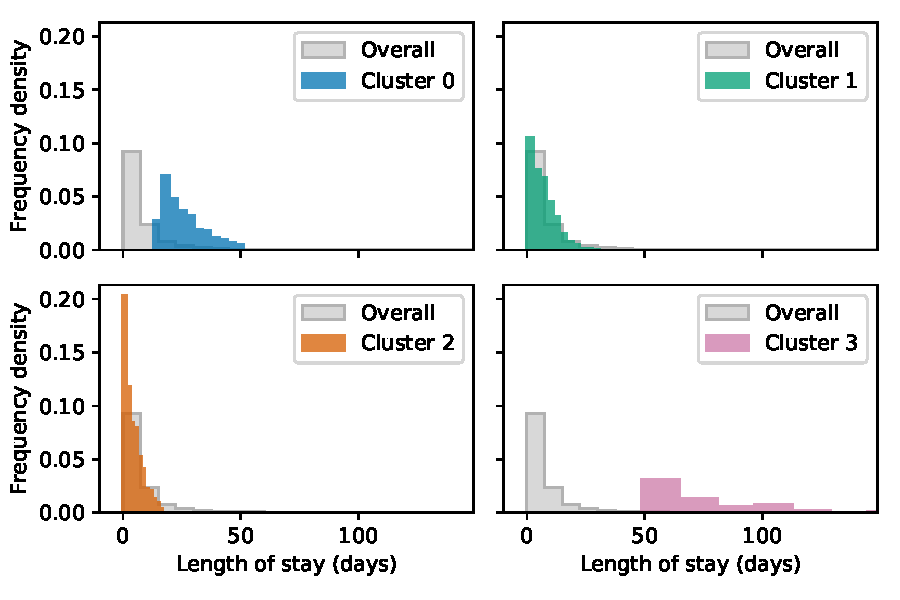
\includegraphics[width=\linewidth]{cluster_true_los}
        \caption{}\label{fig:cluster_los}
    \end{subfigure}\hfill%
    \begin{subfigure}{.5\imgwidth}
        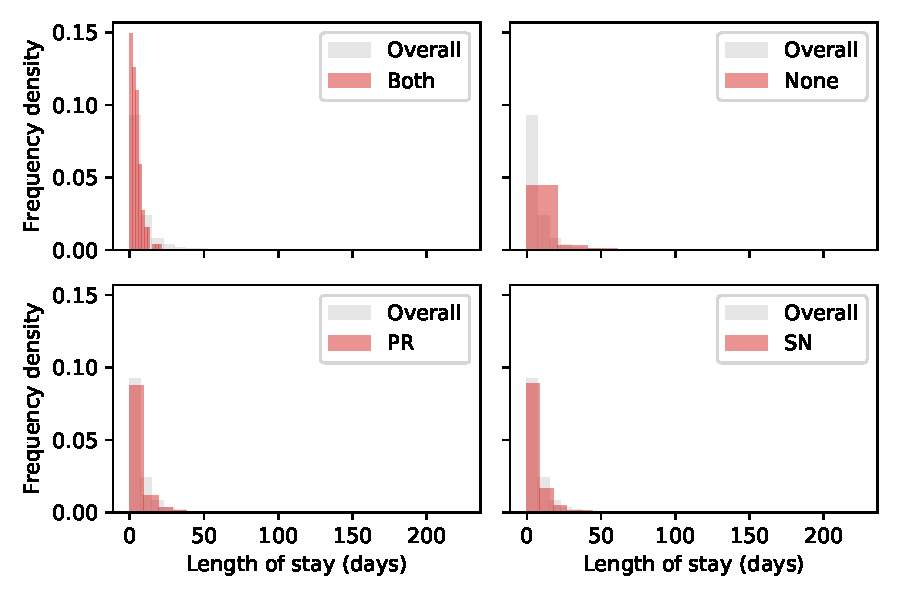
\includegraphics[width=\linewidth]{intervention_true_los}
        \caption{}\label{fig:intervention_los}
    \end{subfigure}
    \caption{%
        Histograms for length of stay by (\subref{fig:cluster_los}) cluster and
        (\subref{fig:intervention_los}) intervention.
    }\label{fig:los}
\end{figure}

\begin{figure}
    \centering
    \begin{subfigure}{.5\imgwidth}
        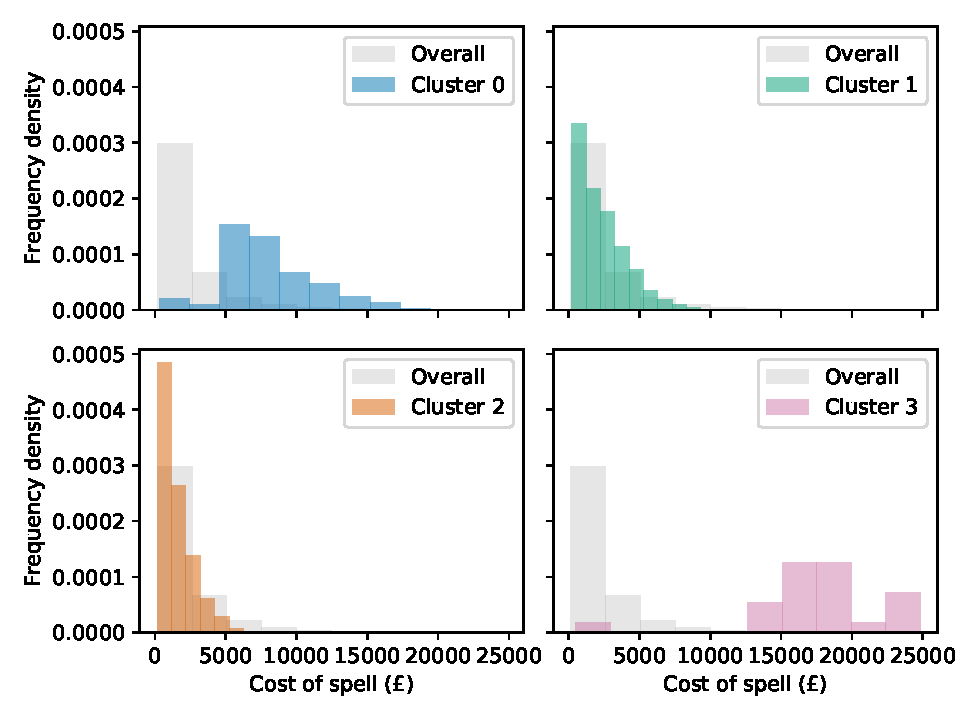
\includegraphics[width=\linewidth]{cluster_spell_cost}
        \caption{}\label{fig:cluster_cost}
    \end{subfigure}\hfill%
    \begin{subfigure}{.5\imgwidth}
        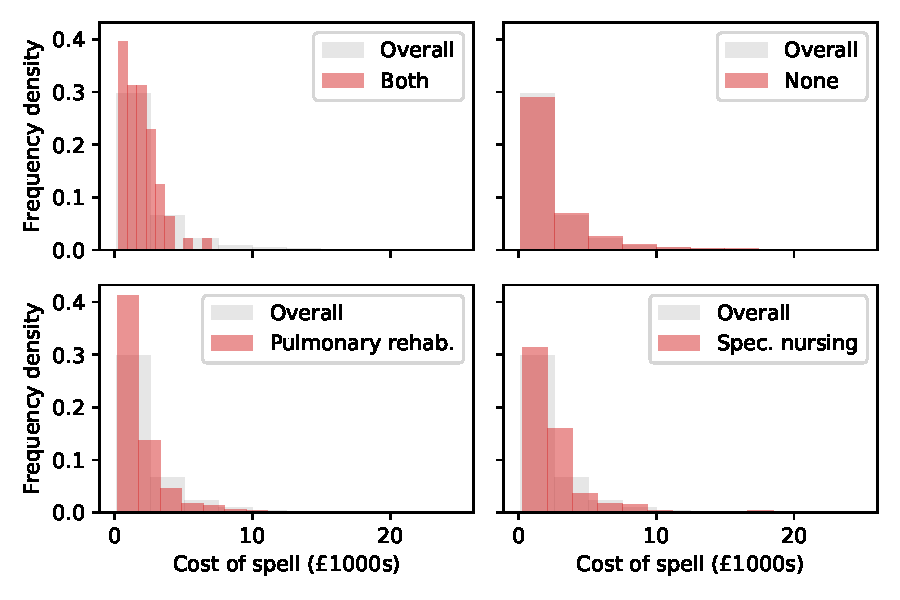
\includegraphics[width=\linewidth]{intervention_spell_cost}
        \caption{}\label{fig:intervention_cost}
    \end{subfigure}
    \caption{%
        Histograms for spell cost by (\subref{fig:cluster_cost}) cluster and
        (\subref{fig:intervention_cost}) intervention.
    }\label{fig:cost}
\end{figure}

Figure~\ref{fig:los} shows the length of stay distributions as histograms.
Figure~\ref{fig:cluster_los} demonstrates the different bed resource
requirements well for each cluster --- better than Table~\ref{tab:summary}
might --- in that the difference between the clusters is not just a matter of
varying means and ranges, but entirely different shapes to their respective
distributions. Indeed, they are all positively skewed but there is no real
consistency beyond that. When comparing this to
Figure~\ref{fig:intervention_los}, there is certainly some variety but the
overall shapes of the distributions are very similar. This is except for the
spells with no COPD intervention where binning could not improve the
visualisation due to the widespread distribution of their lengths of stay.

The same conclusions can be drawn about spell costs from Figure~\ref{fig:cost};
there are distinct patterns between the clusters in terms of their costs, and
they align with the patterns seen in Figure~\ref{fig:los}. This is expected
given that length of stay is a driving force of healthcare costs. Equally, there
is no immediately discernible difference in the distribution of costs even when
splitting by intervention.

\begin{figure}
    \centering
    \begin{subfigure}{.5\imgwidth}
        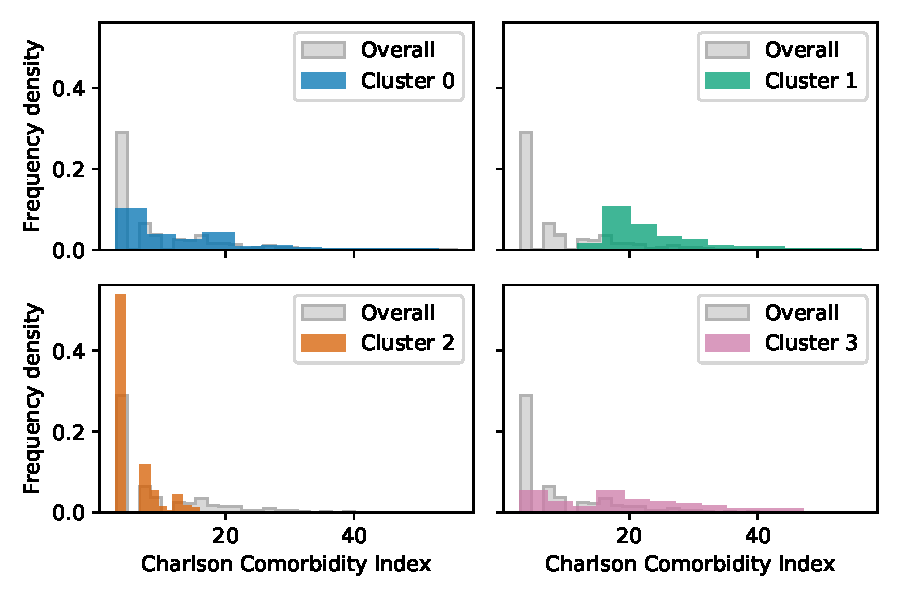
\includegraphics[width=\linewidth]{cluster_charlson_gross}
        \caption{}\label{fig:cluster_charlson}
    \end{subfigure}\hfill%
    \begin{subfigure}{.5\imgwidth}
        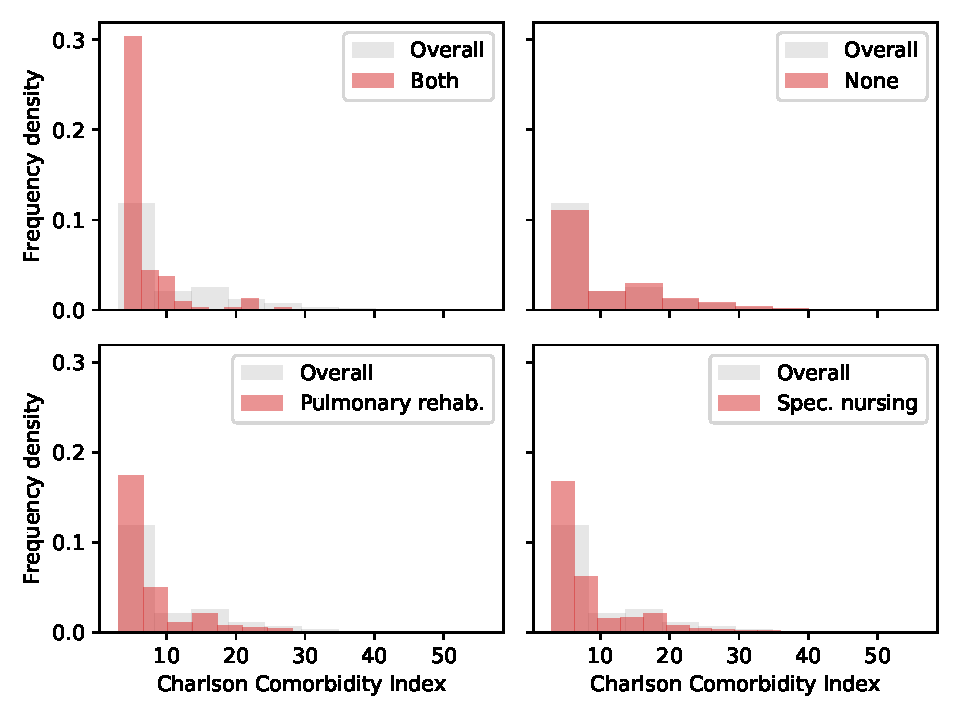
\includegraphics[width=\linewidth]{intervention_charlson_gross}
        \caption{}\label{fig:intervention_charlson}
    \end{subfigure}
    \caption{%
        Histograms for CCI by (\subref{fig:cluster_charlson}) cluster and
        (\subref{fig:intervention_charlson}) intervention.
    }\label{fig:charlson}
\end{figure}

Similarly to the previous figures, Figure~\ref{fig:charlson} shows that
clustering has revealed distinct patterns in the CCI of the spells within each
cluster where splitting by intervention does not. All clusters other than
Cluster 2 show clear, heavy tails, and in the cases of Clusters 1 and 3 the body
of the data exists far from the origin as indicated in Table~\ref{tab:summary}.
In contrast, the plots in Figure~\ref{fig:intervention_charlson} all display
very similar, highly skewed distributions regardless of intervention.

\begin{figure}
    \centering
    \begin{subfigure}{.5\imgwidth}
        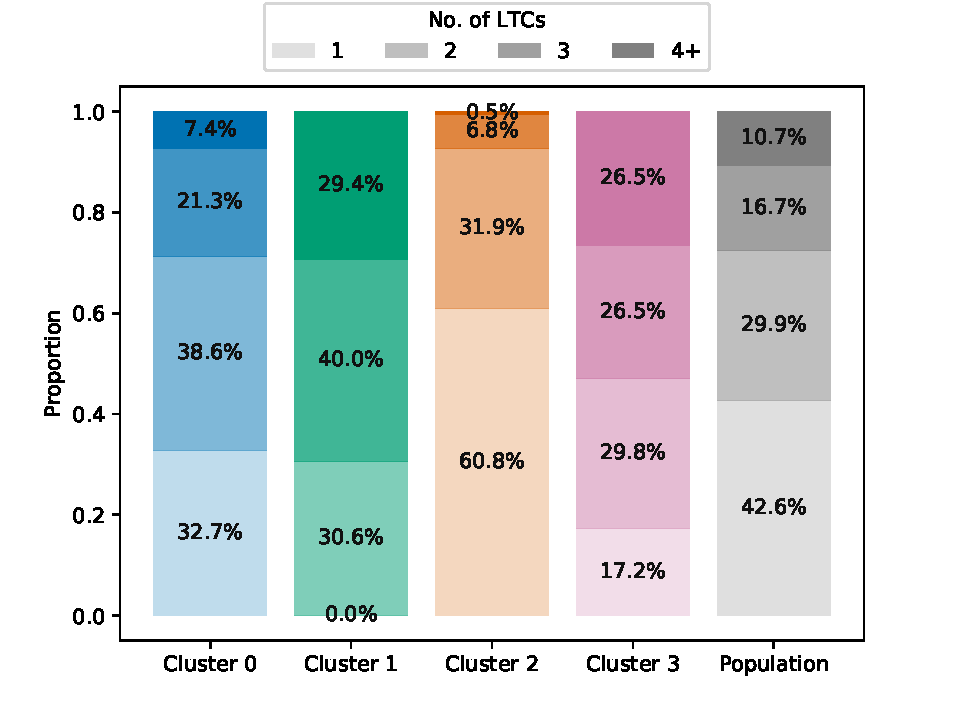
\includegraphics[width=\linewidth]{cluster_ltcs}
        \caption{}\label{fig:cluster_ltcs}
    \end{subfigure}\hfill%
    \begin{subfigure}{.5\imgwidth}
        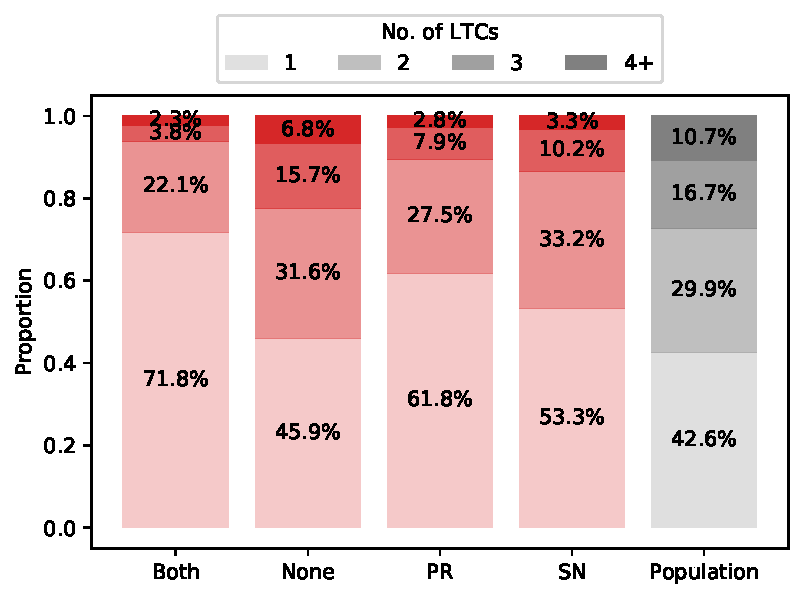
\includegraphics[width=\linewidth]{intervention_ltcs}
        \caption{}\label{fig:intervention_ltcs}
    \end{subfigure}
    \caption{%
        Proportions of the number of concurrent LTCs in a spell by
        (\subref{fig:cluster_ltcs}) cluster and (\subref{fig:intervention_ltcs})
        intervention.
    }\label{fig:ltcs}
\end{figure}

\begin{figure}
    \centering
    \begin{subfigure}{.5\imgwidth}
        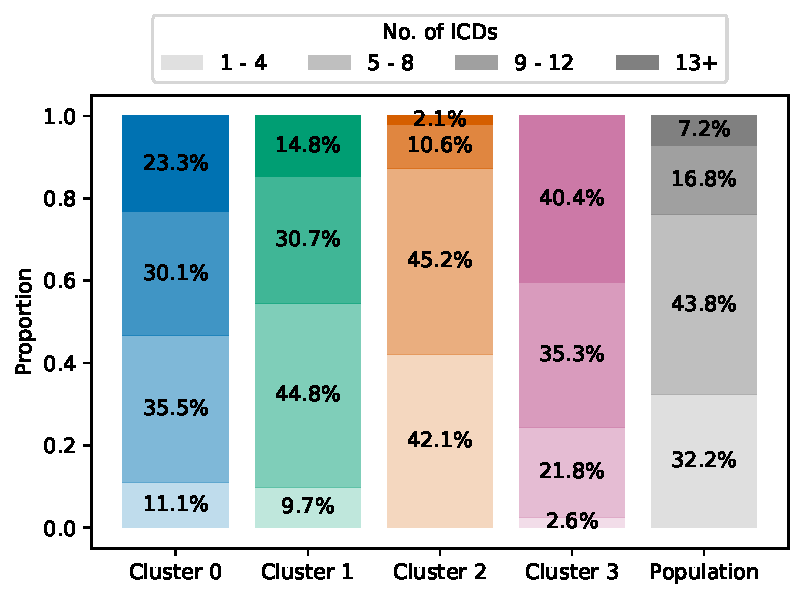
\includegraphics[width=\linewidth]{cluster_icds}
        \caption{}\label{fig:cluster_icds}
    \end{subfigure}\hfill%
    \begin{subfigure}{.5\imgwidth}
        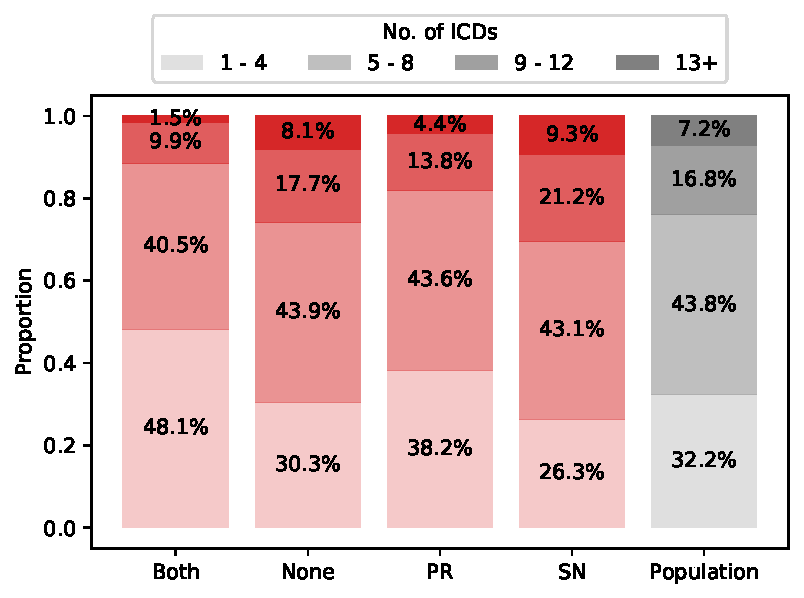
\includegraphics[width=\linewidth]{intervention_icds}
        \caption{}\label{fig:intervention_icds}
    \end{subfigure}
    \caption{%
        Proportions of the number of concurrent ICDs in a spell by
        (\subref{fig:cluster_icds}) cluster and (\subref{fig:intervention_icds})
        intervention.
    }\label{fig:icds}
\end{figure}

Figures~\ref{fig:ltcs}~and~\ref{fig:icds} show the proportions of each grouping
presenting levels of concurrent LTCs and ICDs respectively. By exposing the
distribution of these attributes, some notion of the clinical complexity for
each cluster can be captured better than with Table~\ref{tab:summary} alone. In
Figure~\ref{fig:cluster_ltcs}, for instance, there are distinct LTC count
profiles amongst the clusters: Cluster 0 is typical of the population; Cluster 1
shows that no patient presented solely COPD as an LTC in their spells, and more
than half presented at least three; Cluster 2 is similar in form to the
population but is severely biased towards patients presenting COPD as the only
LTC;\ Cluster 3 is the most uniformly spread amongst the four bins despite
increased length of stay and CCI suggesting a disparate array of patients in
terms of their long term medical needs.

Figure~\ref{fig:cluster_icds} largely mirrors these cluster profiles with the
number of concurrent ICDs. Some points of interest, however, are that Cluster 1
has a relatively low-leaning distribution of ICDs that does not marry up with
the high rates of LTCs, and that the vast majority of spells in Cluster 3
present with at least nine ICDs suggesting a likely wide range of conditions and
comorbidities beyond the LTCs used to calculate CCI.\

When considering the intervention counterparts to these figures (i.e.\
Figures~\ref{fig:intervention_ltcs}~and~\ref{fig:intervention_icds}), very
little can be drawn with regards to the corresponding spells. One thing of note
is that patients receiving both interventions for their COPD (or either, in
fact) have disproportionately fewer LTCs and concurrent ICDs when compared to
the population. Aside from this, the profiles of each intervention are all very
similar to one another.

As discussed earlier, the purpose of this work is to construct a queuing model
for the data described here. Insights have already been gained into the needs of
the segments that have been identified in this section but in order to glean
further insights, some parameters of the queuing model must be recovered from
the data.

\section{Constructing the queuing model}\label{sec:model}

Owing to a lack of available data on the system and its patients, the options
for the queuing model used are limited compared to those employed in some modern
works. However, there is a precedent for simplifying healthcare systems to a
single node with parallel servers that emulate resource
availability.~\cite{Steins2013}~and~\cite{Williams2015} provide good examples of
how this approach, when paired with discrete event simulation, can expose the
resource needs of a system beyond deterministic queuing theory models. In
particular,~\cite{Williams2015} shows how a single node, multiple server queue
can be used to accurately predict bed capacity and length of stay distributions
in a critical care unit using administrative data.

Following in the suit of recent literature, a single node using a \(M/M/c\)
queue is employed to model a hypothetical ward of patients presenting COPD.\ In
addition to this, the grouping found in Section~\ref{subsec:overview} provides
a set of patient classes in the queue. Under this model, the following
assumptions are made:
\begin{enumerate}
    \item Inter-arrival and service times of patients are each exponentially
        distributed with some mean. This is in spite of the system time
        distributions shown in Figure~\ref{fig:cluster_los} in order to
        simplify the model parameterisation.
    \item There are \(c \in \mathbb{N}\) servers available to arriving patients
        at the node representing the overall resource availability including bed
        capacity and hospital staff.
    \item There is no queue or system capacity. In~\cite{Williams2015}, a
        queue capacity of zero is set under the assumption that any surplus
        arrivals would be sent to another suitable ward or unit. As this
        hypothetical ward represents COPD patients potentially throughout a
        hospital, this assumption is not held.
    \item Without the availability of expert clinical knowledge, a first-in
        first-out service policy is employed in lieu of some patient priority 
        framework.
\end{enumerate}

Each group of patients has its own arrival distribution. The parameter of this
distribution is taken to be the reciprocal of the mean inter-arrival times for
that group and is denoted by \(\lambda_i\) for each cluster \(i\).

Like arrivals, each group of patients has its own service time distribution.
Without full details of the process order or idle periods during a spell, some
assumption must be made about the true `service' time of a patient in hospital.
It is assumed here that the mean service time of a group of patients may be
approximated via their mean length of stay, i.e.\ the mean time spent in the
system. For simplicity, this work assumes that for each cluster, \(i\), the mean
service time of that cluster, \(\frac{1}{\mu_i}\), is directly proportional
to the mean total system time of that cluster, \(\frac{1}{\phi_i}\), such that:
\begin{equation}\label{eq:services}
    \mu_i = p_i \phi_i
\end{equation}

\noindent where \(p_i \in \interval[open left]{0}{1}\) is some parameter to be
determined for each group.

One of the few ground truths available in the provided data is the distribution
of the total length of stay. Given that the length of stay and resource
availability are connected, the approach here will be to simulate the length of
stay distribution for a range of values \(p_i\) and \(c\) in order to find the
parameters that best match the observed data. A diagram depicting the process
described in this section is provided in Figure~\ref{fig:process}.

The statistical comparison of two or more distributions can be done in a number
of ways. Such methods include the Kolmogorov-Smirnov test, a variety of
discrepancy approaches such as summed mean-squared error, and \(f\)-divergences.
A popular choice amongst the latter group (which may be considered
distance-like) is the Kullback-Leibler divergence which measures relative
information entropy from one probability distribution to
another~\cite{Kullback1951}. The key issue with many of these methods is that
they lack interpretability which is paramount when conveying information to
stakeholders. Interpretability not just from explaining how something works but
how its results may be explained also.

As such, a reasonable candidate is the (first) Wasserstein metric, also known as
the `earth mover' or `digger' distance~\cite{Vaserstein1969}. The Wasserstein
metric satisfies the conditions of a formal mathematical metric (like the
typical Euclidean distance), and its values take the units of the distributions
under comparison (in this case: days). Both of these characteristics can aid
understanding and explanation. In simple terms, the distance measures the
approximate `minimal work' required to move between two probability
distributions where `work' can be loosely defined as the product of how much of
the distribution's mass is to be moved and the distance it must be moved
by. More formally, the Wasserstein distance between two probability
distributions \(U\) and \(V\) is defined as:
\begin{equation}\label{eq:wasserstein}
    W(U, V) = \int_{0}^{1} \left\vert F^{-1}(t) - G^{-1}(t) \right\vert dt
\end{equation}

\noindent where \(F\) and \(G\) are the cumulative density functions of \(U\)
and \(V\) respectively. A proof of~\eqref{eq:wasserstein} is presented
in~\cite{Ramdas2017}. The parameter set with the smallest maximum distance
between any cluster's simulated system time distribution and the overall
observed length of stay distribution is then taken to be the most appropriate.
To be specific, let \(T\) denote the system time distribution of all of
the observed data and let \(T_{i,c,p}\) denote the system time distribution for
cluster \(i\) obtained from a simulation with \(c\) servers and
\(p := \left(p_0, p_1, p_2, p_3\right)\). Then the optimal parameter set
\(\left(c^*, p^*\right)\) is given by:
\begin{equation}\label{eq:parameters}
    \left(c^*, p^*\right) = \argmin_{c, p} \left\{%
        \max_{i} \left\{ W\left(T_{i,c,p}, T\right) \right\}%
    \right\}
\end{equation}

\begin{figure}
    \centering%
    \resizebox{\imgwidth}{!}{%
        \includestandalone{tex/process}
    }
    \caption{%
        A diagrammatic depiction of the queuing parameter recovery process.
    }\label{fig:process}
\end{figure}

The parameter sweep included values of each \(p_i\) from \(0.5\)
to \(1.0\) with a granularity of \(5.0 \times 10^{-2}\) and values of \(c\) from
\(40\) to \(60\) at steps of \(5\).  These choices were informed by the
assumptions of the model and formative analysis to reduce the parameter space
given the computational resources required to conduct the simulations. Each
parameter set was repeated \(50\) times with each simulation running for four
years of virtual time. The warm-up and cool-down periods were taken to be
approximately one year each leaving two years of simulated data from each
repetition.

\begin{figure}
    \centering%
    \begin{subfigure}{.5\imgwidth}
        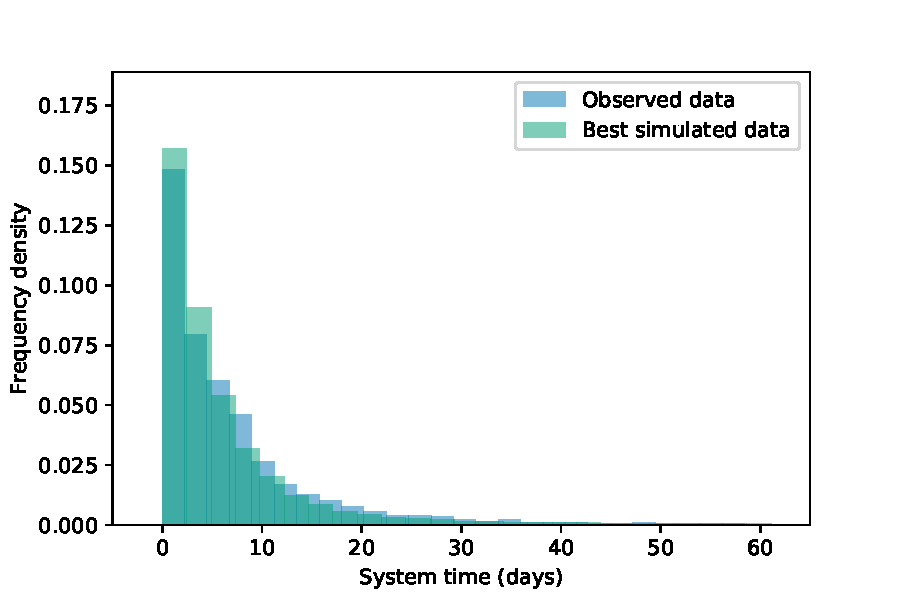
\includegraphics[width=\linewidth]{best_params}
        \caption{}\label{fig:best_params}
    \end{subfigure}\hfill%
    \begin{subfigure}{.5\imgwidth}
        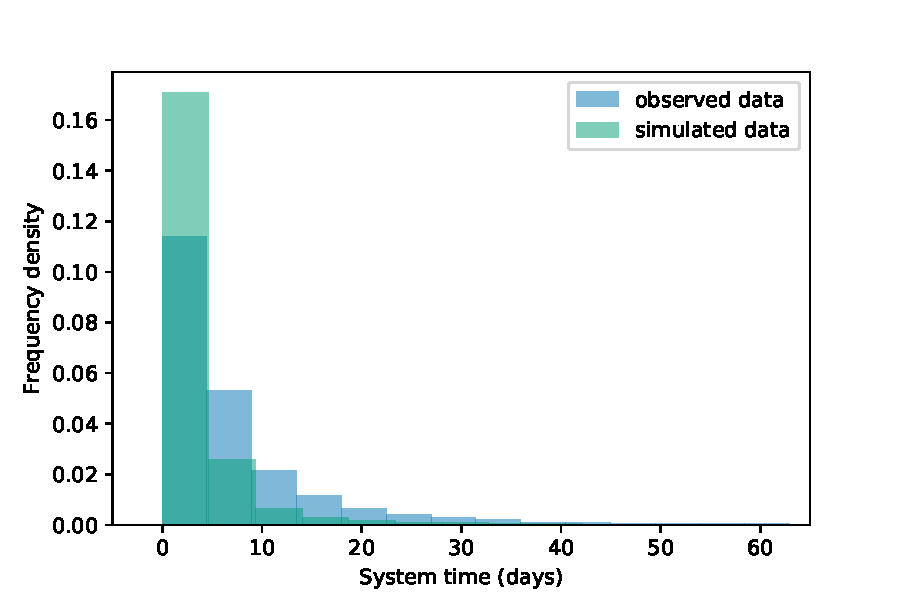
\includegraphics[width=\linewidth]{worst_params}
        \caption{}\label{fig:worst_params}
    \end{subfigure}
    \caption{Histograms of the simulated and observed length of stay data for
             the (\subref{fig:best_params}) best and (\subref{fig:worst_params})
             worst parameter sets.}\label{fig:params}
\end{figure}

The results of this parameter sweep can be summarised in
Figure~\ref{fig:params}. Each plot shows a comparison of the observed lengths
of stay across all groups and the newly simulated data with the best and worst
parameter sets respectively. It can be seen that, in the best case, a very close
fit has been found. Meanwhile, Figure~\ref{fig:worst_params} highlights the
importance of good parameter estimation under this model since the likelihood of
short-stay patient arrivals has been inflated disproportionately against the
tail of the distribution. Table~\ref{tab:comparison} reinforces these results
numerically, showing a clear fit by the best parameters across the board.

\begin{table}
    \centering
    \resizebox{\tabwidth}{!}{\begin{tabular}{lrrrrrrrrrrrrr}
\toprule
{} & \multicolumn{6}{l}{Model parameter and result} & \multicolumn{7}{l}{LOS statistic} \\
{} &                    \(p_0\) & \(p_1\) & \(p_2\) & \(p_3\) & \(c\) & Max. distance &          Mean &   Std. &  Min. &   25\% &  Med. &   75\% &    Max. \\
\midrule
Observed        &                        NaN &     NaN &     NaN &     NaN &   NaN &          0.00 &          7.70 &  11.86 & -0.02 &  1.49 &  4.20 &  8.93 &  224.93 \\
Best simulated  &                        1.0 &     1.0 &     1.0 &     0.5 &  50.0 &          1.30 &          7.11 &  12.41 &  0.00 &  1.44 &  3.55 &  7.64 &  244.46 \\
Worst simulated &                        0.5 &     0.5 &     0.5 &     1.0 &  40.0 &          4.25 &          4.36 &  13.40 &  0.00 &  0.72 &  1.78 &  3.84 &  463.01 \\
\bottomrule
\end{tabular}
}
    \caption{A comparison of the observed data, and the best and worst simulated
        data based on the model parameters and summary statistics for length of
    stay (LOS).}\label{tab:comparison}
\end{table}

In this section, the clustering has been used to enrich the overall queuing
model and to recover the parameters for several classes within that queue to a
high standard. Now, using this model, the next section conducts an investigation
into the underlying system by adjusting the parameters of the queue with the
clustering.

\section{Adjusting the queuing model}\label{sec:scenarios}

This section is comprised of several `what-if' scenarios --- a classic component
of healthcare operational research --- under the novel parameterisation of the
queue established in Section~\ref{sec:model}. The outcomes of interest in this
work are server (resource) utilisation and system times as these metrics capture
the driving forces of cost and flow as well as the overall state of the system,
its staff and its patients. Specifically, the objective of these experiments is
to address the following questions:
\begin{itemize}
    \item How would the system be affected by a change in overall patient
        arrivals?
    \item How is the system affected by a change in resource availability (i.e.\
        a change in \(c\))?
    \item How is the system affected by patients moving between clusters?
\end{itemize}

Owing to the nature of the observed data, the queuing model parameterisation
and its assumptions, the effects on the chosen metrics in each scenario are
given in relative terms with respect to the base case. The base case being those
results generated from the best parameter set recorded in
Table~\ref{tab:comparison}. In particular, the data from each scenario is scaled
by the corresponding median value in the base case meaning that a metric having
a value of 1 is `normal'.

As mentioned in Section~\ref{sec:intro}, the source code used throughout this
work is available online and has been archived. %TODO Add citation for repo
In addition to this, the datasets generated from the simulations in this section
have been archived. %TODO archive and add citation


\subsection{Changes to overall patient arrivals}\label{subsec:arrivals}

Changes in overall patient arrivals to a queue reflect real-world scenarios
where some stimulus is improving (or worsening) the condition of the patient
population. Examples of stimuli could include an aging population or
changes to deprivation. Within this model, overall patient arrivals are altered
using a scaling factor denoted by \(\sigma\in\mathbb{R}\). This scaling factor
is applied to the model by multiplying each cluster's arrival rate by
\(\sigma\). That is, for cluster \(i\), its new arrival rate, \(\hat\lambda_i\),
is given by:
\begin{equation}\label{eq:lambda}
    \hat\lambda_{i} = \sigma\lambda_i
\end{equation}

\begin{figure}
    \centering
    \begin{subfigure}{.5\imgwidth}
        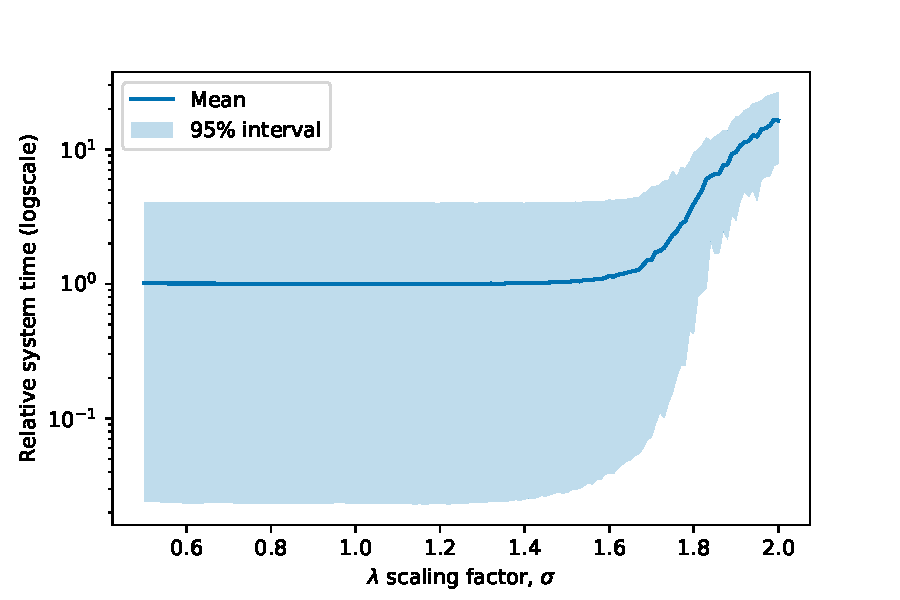
\includegraphics[width=\linewidth]{lambda_time}
        \caption{}\label{fig:lambda_time}
    \end{subfigure}\hfill%
    \begin{subfigure}{.5\imgwidth}
        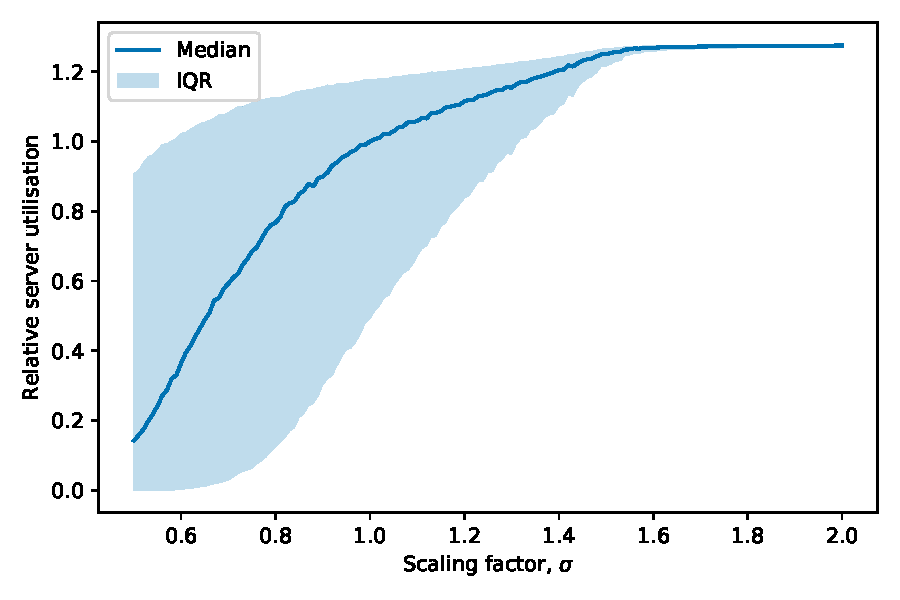
\includegraphics[width=\linewidth]{lambda_util}
        \caption{}\label{fig:lambda_util}
    \end{subfigure}
    \caption{%
        Plots of \(\sigma\) against relative (\subref{fig:lambda_time})~system
        time and (\subref{fig:lambda_util})~server utilisation.
    }\label{fig:lambda}
\end{figure}

Figure~\ref{fig:lambda} shows the effects of changing patient arrivals on
(\subref{fig:lambda_time})~relative system times and
(\subref{fig:lambda_util})~relative server utilisation over values of \(\sigma\)
from 0.5% to 2.0% at a
precision of \(1.0 \times 10^{-2}\)%. Specifically, each plot in the
figure (and the subsequent figures in this section) shows the median and
interquartile range (IQR) of each relative attribute. These metrics provide an
insight into the experience of the average user (or server) in the system, and
in the stability or variation of the body of users (servers).

What is evident from these plots is that things are happening as one might
expect: as arrivals increase, the strain on the system increases. However, it
should be noted that it also appears that the model has some amount of slack
relative to the base case. Looking at Figure~\ref{fig:lambda_time}, for
instance, the relative system times (i.e.\ the relative length of stay for
patients) remains unchanged up to \(\sigma \approx 1.2\), or an approximate 20\%
increase in arrivals of COPD patients. Beyond that, relative system times rise
to an untenable point where the median time becomes orders of magnitude above
the norm.

However, Figure~\ref{fig:lambda_util} shows that the situation for the system's
resources reaches its worst case near to the start of that spike in relative
system times (at \(\sigma \approx 1.4\)). That is, the median server utilisation
reaches a maximum (this corresponds to constant utilisation) at this point and
the variation in server utilisation disappears entirely.


\subsection{Changes to resource availability}\label{subsec:resources}

As is discussed in Section~\ref{sec:model}, the resource availability of the
system is captured by the number of parallel servers in the system, \(c\).
Therefore, to modify the overall resource availability, only the number of
servers need be changed. This kind of sensitivity analysis is usually done to
determine the opportunity cost of adding service capacity to a system, e.g.\
would adding \(n\) servers sufficiently increase efficiency without exceeding
a budget?

To reiterate the beginning of this section, all suitable parameters are given in
relative terms. This includes the number of servers here. By doing this, the
changes in resource availability are more easily seen, and do away with any
concerns as to what a particular number of servers exactly reflects in the real
world.

\begin{figure}
    \centering
    \begin{subfigure}{.5\imgwidth}
        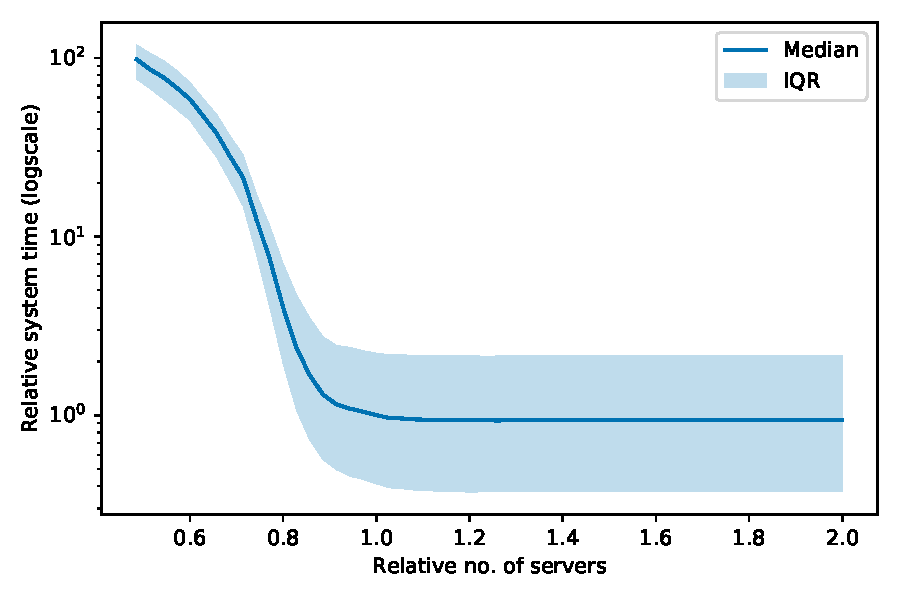
\includegraphics[width=\linewidth]{servers_time}
        \caption{}\label{fig:servers_time}
    \end{subfigure}\hfill%
    \begin{subfigure}{.5\imgwidth}
        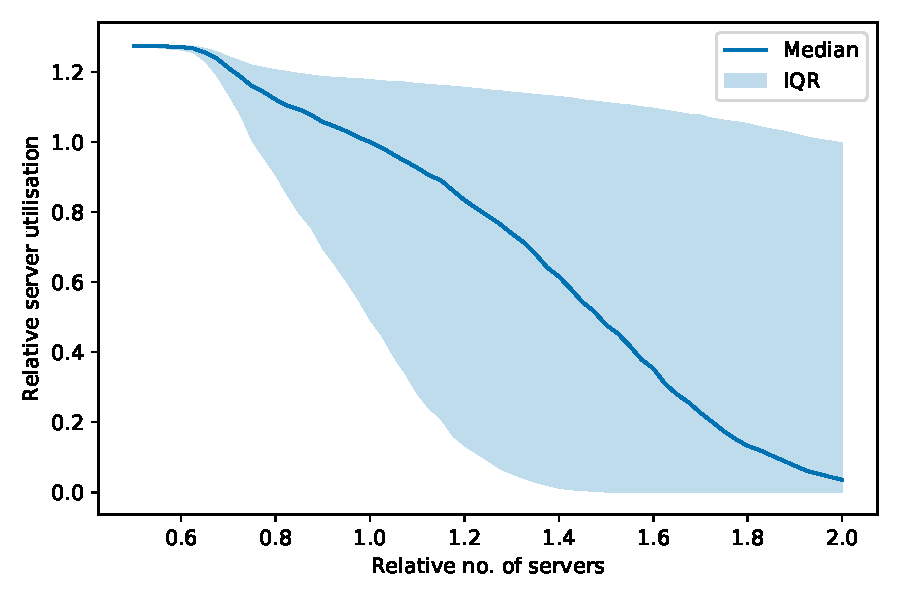
\includegraphics[width=\linewidth]{servers_util}
        \caption{}\label{fig:servers_util}
    \end{subfigure}
    \caption{%
        Plots of the relative number of servers against relative
        (\subref{fig:servers_time})~system time and
        (\subref{fig:servers_util})~server utilisation.
    }\label{fig:servers}
\end{figure}

Figure~\ref{fig:servers} shows how the relative resource availability affects
relative system times and server utilisation. In this scenario, the relative
number of servers took values from 0.5% to
2.0% at steps of
\(2.9 \times 10^{-2}\)% --- this is equivalent to a step size of 1
in the actual number of servers. Overall, these figures fortify the
claim from the previous scenario that there is some room to manoeuvre so that
the system runs `as normal' but pressing on those boundaries results in massive
changes to both resource requirements and system times.

In Figure~\ref{fig:servers_time} this amounts to a maximum of 20\% slack in
resources before relative system times are affected; further reductions quickly
result in a potentially tenfold increase in the median system time, and up to 50
times once resource availability falls by 50\%. Moreover, the variation in the
body of the relative times (i.e.\ the IQR) decreases as resource availability
decreases. The reality of this is that patients arriving at a hospital are
forced to consume larger amounts of resources (simply by being in a hospital)
regardless of their condition, putting added strains on the system.

Meanwhile, it appears that there is no tangible change in relative system times
given an increase in the number of servers. This indicates that the model
carries sufficient resources to cater to the population under normal
circumstances, and that adding service capacity will not necessarily improve
system times.

Again, Figure~\ref{fig:servers_util} shows that there is a substantial change in
the variation in the relative utilisation of the servers. In this case, the
variation dissipates as resource levels fall and increases as they increase.
While the relationship between real hospital resources and the number of servers
is not exact, having variation in server utilisation would suggest that parts of
the system may be configured or partitioned away in the case of some significant
public health event (such as a global pandemic) without overloading the system.


\subsection{Moving arrivals between clusters}\label{subsec:moving}

This scenario is perhaps the most relevant to actionable public health research
of those presented here. The clusters identified in this work could be
characterised by their clinical complexities and resource requirements, as done
in Section~\ref{subsec:overview}. Therefore, being able to model the movement of
some proportion of patient spells from one cluster to another will reveal how
those complexities and requirements affect the system itself. The reality is
then that if some public health policy could be implemented to enact that
movement informed by a model such as this then real change would be seen in the
real system.

In order to model the effects of spells moving between two clusters, the
assumption is that services remain the same (and so does each cluster's \(p_i\))
but their arrival rates are altered according to some transfer proportion.
Consider two clusters indexed at \(i, j\), and their respective arrival rates,
\(\lambda_i, \lambda_j\), and let \(\delta \in [0, 1]\) denote the proportion of
arrivals to be moved from cluster \(i\) to cluster \(j\). Then the new arrival
rates for each cluster, denoted by \(\hat\lambda_i, \hat\lambda_j\)
respectively, are:
\begin{equation}\label{eq:moving}
    \hat\lambda_i = \left(1 - \delta\right) \lambda_i
    \quad \text{and} \quad
    \hat\lambda_j = \delta\lambda_i + \lambda_j
\end{equation}

By moving patient arrivals between clusters in this way, the overall arrivals
are left the same since the sum of the arrival rates is the same. Hence, the
(relative) effect on server utilisation and system time can be measured
independently.

Figures~\ref{fig:moving_time}~and~\ref{fig:moving_util} show the effect of
moving patient arrivals between clusters on relative system time and relative
server utilisation respectively. In each figure, the median and IQR for the
corresponding attribute is shown, as in the previous scenarios. Each scenario
was simulated using values of \(\delta\) from 0.0% to
1.0% at steps of \(1.0 \times 10^{-1}\)%.

Considering Figure~\ref{fig:moving_time}, it is clear that there are some cases
where reducing particular types of spells (by making them like another type of
spell) has no effect on overall system times. Namely, moving the high
resource requirement spells that make up Cluster 0 and Cluster 3 to any other
cluster. These clusters make up only 10\% of all arrivals and this figure shows
that in terms of system times the model is able to handle them without concern
under normal conditions. The concern comes when either of the other clusters
moves to Cluster 0 or Cluster 3. Even as few as one in five of the low
complexity, low resource needs arrivals in Cluster 2 moving to either cluster
results in large jumps in the median system time for all arrivals, and soon
after, as in the previous scenario, any variation in the system times
disappears indicating an overborne system.

With relative server utilisation, the story is much the same. The normal levels
of high complexity, high resource arrivals from Cluster 3 are absorbed by the
system and moving these arrivals to another cluster bears no effect on resource
consumption levels. Likewise, either of the low resource need clusters moving
even slightly toward high resource requirements completely overruns the system's
resources. However, the relative utilisation levels of the system resources can
be reduced by moving arrivals from Cluster 0 to either Cluster 1 or Cluster 2,
i.e.\ by reducing the overall resource requirements of such spells.

In essence, these figures offer two messages: that while some hard spells are
inevitable, they are manageable under the current state of the system, and that
public health policy informed by this model should be preventative in nature. If
an effective policy could be implemented to reduce the resource requirements of
COPD patients when they arrive at a hospital --- for instance, by increasing
access to community care or campaigns against harmful behaviours such as smoking
--- then lengths of stay and strains on the hospital's resources would be
reduced, improving the system as a whole.

\begin{figure}
    \centering
    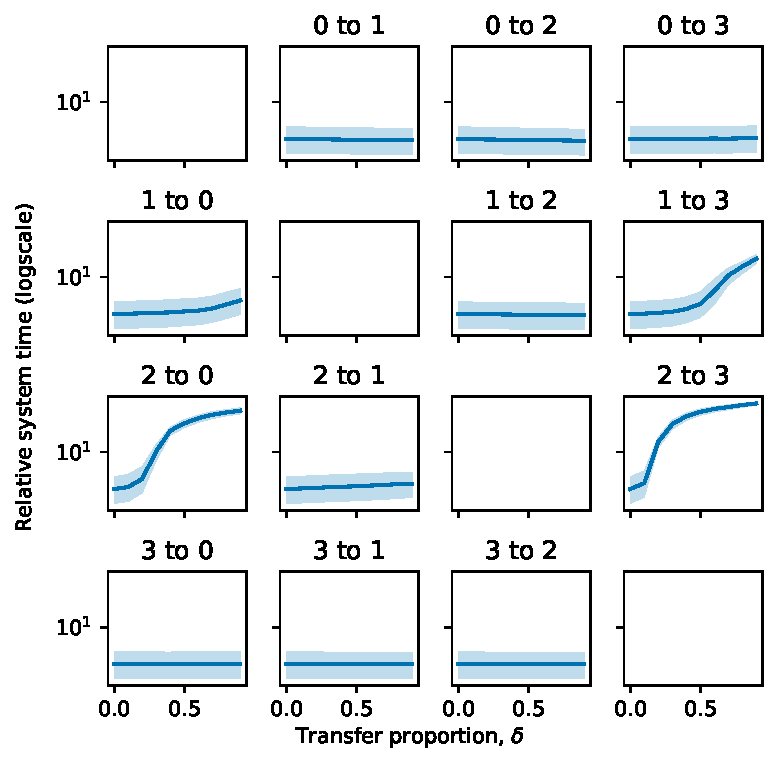
\includegraphics[width=\imgwidth]{moving_time}
    \caption{%
        Plots of proportions of each cluster moving to another against relative
        system time.
    }\label{fig:moving_time}
\end{figure}

\begin{figure}
    \centering
    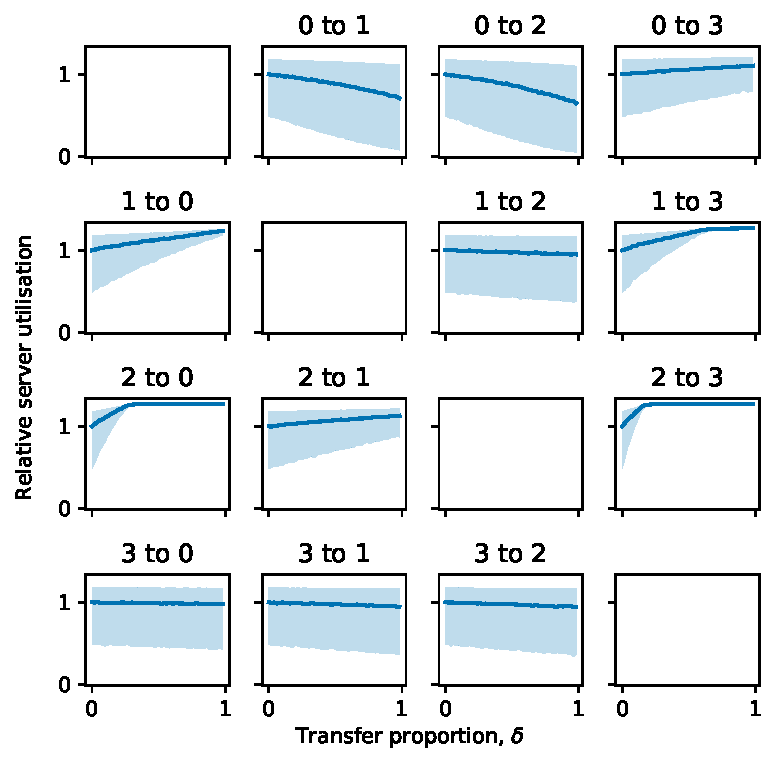
\includegraphics[width=\imgwidth]{moving_util}
    \caption{%
        Plots of proportions of each cluster moving to another on relative
        server utilisation.
    }\label{fig:moving_util}
\end{figure}

\section{Conclusion}\label{sec:conclusion}

This work presents a novel approach to investigating a healthcare population
that encompasses the topics of segmentation analysis, queuing models, and the
recovery of queuing parameters from incomplete data. This is done despite common
limitations in operational research with regard to the availability of
fine-grained data, and this work only uses administrative hospital spell data
from patients presenting COPD in the South Wales area.\

By considering a variety of attributes present in the data, and engineering
some, an effective clustering of the spell population is identified that
successfully feeds into a multi-class, \(M/M/c\) queue to model a hypothetical
COPD ward. With this model, a number of insights are gained by investigating
purposeful changes in the parameters of the model that have the potential to
inform actual public health policy.

In particular, since neither the resource capacity of the system or the clinical
processes of the spells are evident in the data, service times and resource
levels are not available. However, length of stay is. Using what is available,
this work assumes that mean service times can be parameterised using mean
lengths of stay. By using the Wasserstein distance to compare the distribution
of the simulated lengths of stay data with the observed data, a best performing
parameter set is found via a parameter sweep.

This parameterisation ultimately recovers a surrogate for service times for each
cluster, and a common number of servers to emulate resource availability. The
parameterisation itself offers its strengths by being simple and effective.
Despite its simplicity, a good fit to the observed data is found, and --- as is
evident from the closing section of this work --- substantial and useful
insights can be gained into the needs of the COPD patient population being
studied.


\bibliography{bibliography}

\end{document}
